\section{Modelo de dados em HL7 FHIR}
\label{sec:modelo-fhir}

Esta seção corresponde às etapas 5 e 6 do trabalho (Seção~\ref{sec:etapas}). A CIF foi modelada em detalhe, com
instâncias de exemplo validadas, e os outros seis formulários foram analisados quanto à estrutura, conforme o
recorte descrito na introdução. Os artefatos da CIF são gerados a partir do catálogo e da calculadora do aplicativo
pelo script \arq{entregas/scripts/gerar_fhir_cif.py} e ficam no diretório \arq{entregas/fhir/cif/}, no repositório
do TCC.

\subsection{Escolhas de modelagem}
\label{sec:fhir-escolhas}

O modelo usa o FHIR R4 (4.0.1), os perfis do BR-Core 1.7.1 e as extensões do SDC 4.0.0
(\citeauthor{brcore2026}, \citeyear{brcore2026}; \citeauthor{hl7fhirR4}, \citeyear{hl7fhirR4}, \citeyear{hl7sdc}). O paciente e o avaliador seguem os perfis \textit{Patient} e
\textit{Practitioner} do BR-Core, enquanto os resultados por capítulo e por área seguem o perfil \textit{Observation}.
Como o BR-Core não tem perfil de formulário (Seção~\ref{sec:ref-fhir}), o \textit{Questionnaire} e o
\textit{QuestionnaireResponse} usam os recursos-base do R4. Nenhuma extensão ou perfil próprio foi necessário. Os
artefatos próprios (o sistema de códigos e o questionário) têm o endereço canônico provisório
\texttt{https://bemtevi.unb.br/fhir} e a versão 0.1.0.

A Figura~\ref{fig:fhir-conceitual} mostra o modelo conceitual da avaliação, que corresponde ao modelo de informação
da Portaria 1.434/2020 (Seção~\ref{sec:ref-fhir}), com cada entidade representada por um recurso do FHIR. O
instrumento e os seus itens descrevem a estrutura do formulário como dado: o tipo de cada item, os valores
permitidos, a condição de exibição e a regra de cálculo. A avaliação é a aplicação de uma versão do instrumento a um
paciente, por um profissional, e contém uma resposta para cada item habilitado. Os resultados são obtidos das
respostas e, na CIF, são agrupados por capítulo e por área. O modelo é o mesmo para os sete formulários, e o que
muda entre eles são os itens e as regras de cálculo. Nos outros seis formulários, os valores calculados ficam, nesta
etapa, como respostas somente leitura (Seção~\ref{sec:fhir-cobertura}). O dicionário de dados, com o
significado, a unidade e os valores permitidos de cada campo, depende da equipe e fica para o TCC 2.

\begin{figure}[htb]
	\centering
	\caption{Modelo conceitual da avaliação e recursos do HL7 FHIR que o representam}
	\label{fig:fhir-conceitual}
	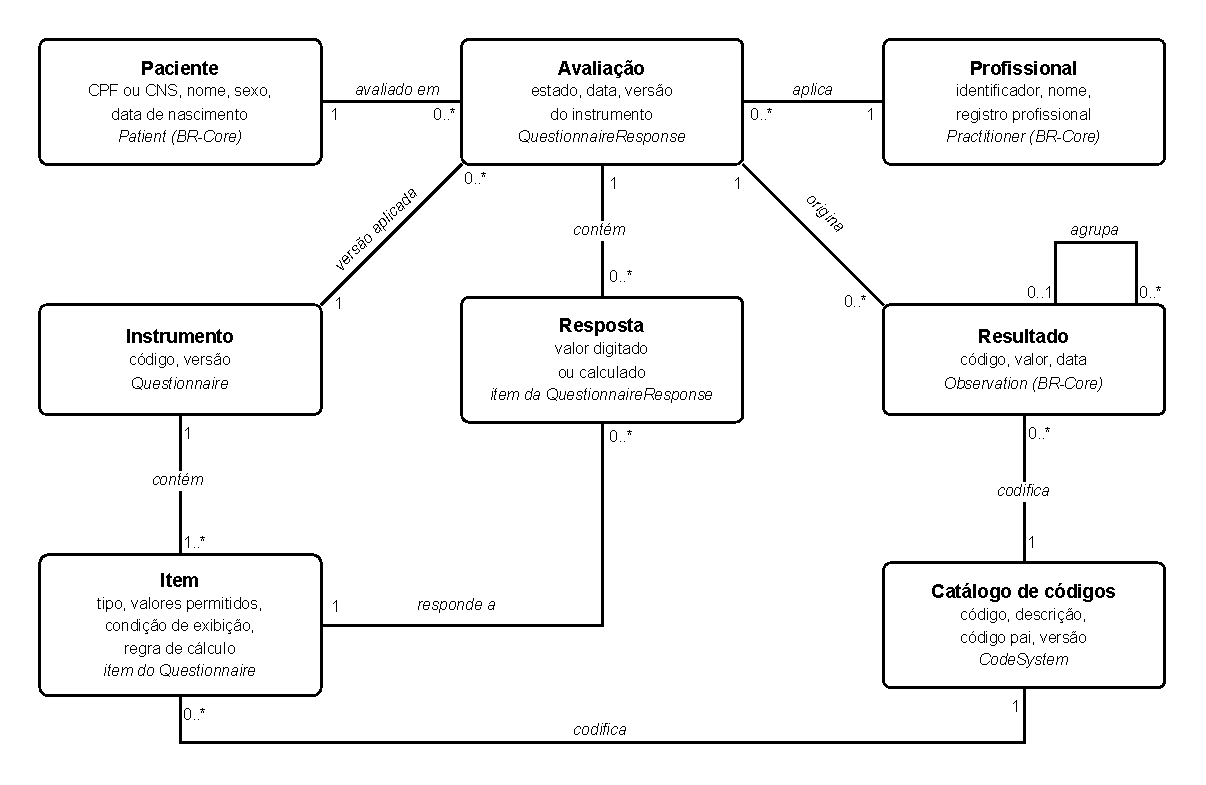
\includegraphics[width=\textwidth]{figuras/modelo-conceitual-fhir.pdf}
	% Versão anterior em TikZ, mantida para referência:
	% \begin{tikzpicture}[
	% font=\footnotesize,
	% entidade/.style={draw, rounded corners=2pt, align=center, text width=3.3cm, inner sep=3pt},
	% rel/.style={semithick},
	% card/.style={font=\scriptsize, inner sep=1.5pt},
	% rotulo/.style={font=\scriptsize\itshape, inner sep=1.5pt},
	% ]
	% \newcommand{\ent}[3]{\textbf{#1}\\[1pt]{\scriptsize #2}\\[2pt]{\scriptsize\textit{#3}}}
	% \node[entidade] (pac) at (0,0) {\ent{Paciente}{CPF ou CNS, nome, sexo,\\data de nascimento}{Patient (BR-Core)}};
	% \node[entidade] (ava) at (5.2,0) {\ent{Avaliação}{estado, data, versão\\do instrumento}{QuestionnaireResponse}};
	% \node[entidade] (pro) at (10.4,0) {\ent{Profissional}{identificador, nome,\\registro profissional}{Practitioner (BR-Core)}};
	% \node[entidade] (ins) at (0,-3.3) {\ent{Instrumento}{código, versão}{Questionnaire}};
	% \node[entidade] (res) at (5.2,-3.3) {\ent{Resposta}{valor digitado\\ou calculado}{item da QuestionnaireResponse}};
	% \node[entidade] (rst) at (10.4,-3.3) {\ent{Resultado}{código, valor, data}{Observation (BR-Core)}};
	% \node[entidade] (ite) at (0,-6.6) {\ent{Item}{tipo, valores permitidos,\\condição de exibição,\\regra de cálculo}{item do Questionnaire}};
	% \node[entidade] (cat) at (10.4,-6.6) {\ent{Catálogo de códigos}{código, descrição,\\código pai, versão}{CodeSystem}};
	% 
	% % Avaliação
	% \draw[rel] (pac) -- node[rotulo, above] {avaliado em} node[card, pos=0.14, below] {1} node[card, pos=0.84, below] {0..*} (ava);
	% \draw[rel] (pro) -- node[rotulo, above] {aplica} node[card, pos=0.14, below] {1} node[card, pos=0.84, below] {0..*} (ava);
	% \draw[rel] (ins.north east) -- node[rotulo, sloped, above] {versão aplicada} node[card, pos=0.1, below right] {1} node[card, pos=0.88, below right] {0..*} (ava.south west);
	% \draw[rel] (ava) -- node[rotulo, fill=white] {contém} node[card, pos=0.15, right] {1} node[card, pos=0.82, right] {0..*} (res);
	% \draw[rel] (ava.south east) -- node[rotulo, sloped, above] {origina} node[card, pos=0.1, below left] {1} node[card, pos=0.88, below left] {0..*} (rst.north west);
	% % Instrumento e itens
	% \draw[rel] (ins) -- node[rotulo, fill=white] {contém} node[card, pos=0.15, right] {1} node[card, pos=0.82, right] {1..*} (ite);
	% \draw[rel] (res.south) |- node[rotulo, pos=0.75, above] {responde a} node[card, pos=0.1, right] {0..*} node[card, pos=0.96, above] {1} (ite.east);
	% % Códigos
	% \draw[rel] (cat) -- node[rotulo, fill=white] {codifica} node[card, pos=0.15, right] {1} node[card, pos=0.82, right] {0..*} (rst);
	% \draw[rel] (cat.south) -- ++(0,-5mm) -| node[rotulo, pos=0.25, below] {codifica} node[card, pos=0.04, below] {1} node[card, pos=0.8, right] {0..*} (ite.south);
	% % Agrupamento dos resultados
	% \draw[rel] ([xshift=-12mm]rst.north east) -- ++(0,5mm) -- node[rotulo, above] {agrupa} ++(8mm,0) -- ++(0,-5mm);
	% \node[card, anchor=south east] at ([xshift=-12mm]rst.north east) {0..1};
	% \node[card, anchor=south west] at ([xshift=-4mm]rst.north east) {0..*};
	% \end{tikzpicture}
	\fonte{Elaborada pelo autor. Em itálico, o recurso ou elemento do FHIR R4 que representa a entidade. ``Agrupa'':
	na CIF, o resultado da área agrupa os resultados dos capítulos (\textit{hasMember}).}
\end{figure}

O Quadro~\ref{qua:fhir-cif} liga cada elemento do módulo CIF ao
elemento do modelo que o representa e aos requisitos da Seção~\ref{sec:especificacao} que ele atende.

\begin{quadro}[H]
	\centering
	\caption{Elementos do módulo CIF no modelo em HL7 FHIR}
	\label{qua:fhir-cif}
	\footnotesize
	\begin{tabularx}{\textwidth}{|>{\raggedright\arraybackslash}p{0.22\textwidth}|>{\raggedright\arraybackslash}X|>{\raggedright\arraybackslash}p{0.17\textwidth}|}
		\hline
		Módulo CIF & Modelo em FHIR & Requisitos \\ \hline
		Catálogo (\arq{catalogo.v0.1.json}) & \textit{CodeSystem} próprio, com 1.452 códigos, o pai de cada código e as
			pendências da planilha & RN08, RNF01 \\ \hline
		Formulário de cada sexo & Um único \textit{Questionnaire}; o sexo vem do cadastro e habilita, por
			\textit{enableWhen}, os 44 itens exclusivos de um dos sexos & RF01, RN05 \\ \hline
		Item digitado (1.007) & Item \textit{integer} obrigatório, com mínimo 0 e máximo 4 & RN01 \\ \hline
		Item calculado (230) & Item \textit{decimal} somente leitura, com a média declarada em
			\textit{calculatedExpression} & RN02, RN03, RN04, RN06, RN07 \\ \hline
		Avaliação & \textit{QuestionnaireResponse}, com o estado e a versão do questionário & RF02, RF04, RNF01 \\ \hline
		Paciente & \textit{Patient} (BR-Core), referenciado em \textit{subject} & RF08, RNF09 \\ \hline
		Avaliador & \textit{Practitioner} (BR-Core), referenciado em \textit{author} & RF09 \\ \hline
		Resultado por capítulo e área & \textit{Observation} (BR-Core); a da área agrupa as dos capítulos com
			\textit{hasMember}, e todas apontam para as respostas com \textit{derivedFrom} & RF05, RF07, RN09, RN11 \\ \hline
	\end{tabularx}
	\fonte{Elaborado pelo autor a partir dos artefatos de \arq{entregas/fhir/cif/}.}
\end{quadro}

Algumas regras do módulo não são representadas pelo modelo e continuam a cargo do servidor. É o caso da proibição de
editar uma avaliação concluída (RN10) e do bloqueio do registro durante o recálculo (RNF03). O FHIR registra o estado
da resposta, mas não impede, por si, a alteração de um recurso concluído.

\subsection{A CIF no modelo}
\label{sec:fhir-cif}

\textbf{Sistema de códigos.} O catálogo virou um \textit{CodeSystem} próprio, versionado, com 1.452 códigos, cada um
com a descrição da planilha e o código pai. Não basta usar a CIF publicada pela OMS. O HL7 Terminology registra a URI
da CIF, mas não traz os códigos \cite{hl7tho2025icf}. As descrições do aplicativo foram tiradas da planilha da
equipe, em português, e não da tradução oficial. E a planilha tem códigos que não podem ser copiados como estão. O
catálogo tem 1.455 nós, e o \textit{CodeSystem}, que não admite código repetido, tem 1.452 códigos. Três códigos
aparecem em duas linhas cada (s73020, d335 e e5151), e a linha 263 de Fatores Ambientais traz o código e598, que
também está na linha 269, embora o título da linha seja o de e595 (RN08). O modelo usa e595, assim como a
calculadora, e os quatro casos ficam marcados em uma propriedade de pendência, para a equipe decidir. Na primeira
versão, as \textit{Observation} traziam também o código da CIF no HL7 Terminology, mas o validador avisou que esse
sistema exige a versão da CIF, que a planilha não informa. Esse código foi retirado, e a ligação com a CIF publicada
fica como pendência (Seção~\ref{sec:consolidacao}).

\textbf{Questionário.} Um único \textit{Questionnaire} cobre os dois sexos, com um grupo para cada área e, dentro
dele, um grupo para cada capítulo. Cada item é identificado pela área e pela célula da planilha, como
\texttt{b:E105}, e não pelo código, porque o código se repete em alguns casos. O questionário tem 1.237 itens de
dados, os mesmos que a calculadora alcança em algum dos sexos: 1.007 digitados e 230 calculados. Além deles, há o
sexo e a data da avaliação, que corresponde à coluna \arq{data_avaliacao} da tabela da CIF. A única célula com
fórmula que fica de fora, s:E211, também fica fora da cadeia de fórmulas da calculadora. Os itens digitados são
inteiros obrigatórios, de 0 a 4 (RN01). O tipo \textit{choice} com \textit{ordinalValue} permitiria mostrar a
descrição de cada qualificador e acomodaria também os qualificadores 8 e 9 (RN33), mas o inteiro é mais simples e
corresponde à regra atual. Os itens calculados são somente leitura (RN06) e declaram a média em uma
\textit{calculatedExpression} (RN02). A Figura~\ref{fig:fhir-b167} mostra o item do exemplo condutor, que usa a
fórmula corrigida na auditoria (RN07).

\begin{figure}[H]
	\centering
	\caption{Item calculado do b167 no \textit{Questionnaire} da CIF}
	\label{fig:fhir-b167}
	\begin{minipage}{\textwidth}
	\scriptsize
\begin{verbatim}
{
  "linkId": "b:E105",
  "code": [ { "system": "https://bemtevi.unb.br/fhir/CodeSystem/cif-catalogo",
              "code": "b167" } ],
  "text": "b167 Funções mentais da linguagem",
  "type": "decimal",
  "readOnly": true,
  "extension": [ {
    "url": "http://hl7.org/fhir/uv/sdc/StructureDefinition/
            sdc-questionnaire-calculatedExpression",
    "valueExpression": {
      "description": "Média; fórmula usada pelo calculador do app:
                      AVERAGE(E106,E112,E118,E119)",
      "language": "text/fhirpath",
      "expression": "(%resource.repeat(item).where(linkId = 'b:E106').answer.value
                    + %resource.repeat(item).where(linkId = 'b:E112').answer.value
                    + %resource.repeat(item).where(linkId = 'b:E118').answer.value
                    + %resource.repeat(item).where(linkId = 'b:E119').answer.value) / 4"
    } } ]
}
\end{verbatim}
	\end{minipage}
	\fonte{Elaborada pelo autor; trecho de \arq{entregas/fhir/cif/Questionnaire-cif.json}.}
\end{figure}

A expressão soma as respostas citadas na fórmula, termo a termo, e divide o total pelo número de termos. A soma termo
a termo, sem filtrar o conjunto de respostas, preserva a referência repetida, como a de E119 antes da correção. Em
FHIRPath, a soma com um operando vazio resulta vazia. Assim, se faltar uma resposta, o item calculado fica sem valor,
e o vazio sobe pela cadeia até a área, como a pendência da calculadora (RN03). A expressão não arredonda o resultado
(RN04).

O sexo é um item somente leitura, preenchido a partir do cadastro (\textit{Patient.gender}) por uma
\textit{initialExpression}, com o paciente declarado como contexto do formulário. Os 33 itens que aparecem só no
formulário feminino e os 11 que aparecem só no masculino, sejam digitados ou calculados, têm um \textit{enableWhen}
sobre esse item (RN05). O cadastro do aplicativo também aceita o sexo ``Outro'' (\arq{pacienteCadastro.dart}, linha
256). Nesse caso, e quando o sexo não é informado, o item fica sem resposta e, como é obrigatório, a avaliação não
pode ser concluída. O resultado é o mesmo da calculadora, que mantém a avaliação pendente sem o sexo e a rejeita
quando o sexo é diferente de masculino ou feminino (\arq{calculador.py}, linhas 724--734).

\textbf{Respostas e resultados.} Cada avaliação é registrada em um \textit{QuestionnaireResponse}, que aponta para o
paciente, para o avaliador e para o questionário com a sua versão (RNF01). Uma resposta em rascunho tem o estado
\textit{in-progress}, e o SDC só permite o estado \textit{completed} quando todos os itens obrigatórios habilitados
têm resposta, a mesma condição de conclusão do aplicativo (RF02 e RF04). O exemplo condutor é uma avaliação fictícia
de um paciente masculino, com as notas do grupo b167 da Figura~\ref{fig:cif-b167} e 0 nos demais itens. Além do sexo
e da data, ela tem 1.204 respostas: 984 digitadas e 220 calculadas, com os valores da calculadora do aplicativo.
Nela, o b167 vale 2,625. Os resultados por capítulo e por área ficam em 34 \textit{Observation}, uma para cada um dos
30 capítulos e uma para cada área, com o valor exibido pelo aplicativo, de duas casas decimais. A
\textit{Observation} da área agrupa as dos seus capítulos com \textit{hasMember}, e não há \textit{Observation} acima
das áreas, porque a avaliação não tem resultado geral (RN09). Todas apontam, com \textit{derivedFrom}, para a resposta
de que foram obtidas e usam o código do capítulo ou da área no sistema próprio. Com isso, a comparação entre duas
avaliações (RF07) pode ser feita sobre as \textit{Observation} de mesmo código, de avaliações respondidas na mesma
versão do questionário (RN11).

No modelo da CIF, o valor ausente só aparece no rascunho: o item sem nota fica sem resposta, e os itens calculados que
dependem dele ficam sem valor. Como as \textit{Observation} só são geradas a partir de uma avaliação concluída, em que
todas as notas existem, o modelo atual da CIF não precisa do \textit{dataAbsentReason}. Ele passa a ser necessário se
a equipe decidir registrar os qualificadores 8 e 9 (RN33), que indicam item não especificado e item que não se
aplica, e serve também para o índice de acomodação do eletrodiagnóstico, hoje gravado como o texto ``N/A'' quando
falta um dado (RN16).

\subsection{Verificação}
\label{sec:fhir-verificacao}

Os 39 arquivos de \arq{entregas/fhir/cif/}, com o sistema de códigos, o questionário, o paciente, o avaliador, as
respostas e as 34 \textit{Observation}, passaram no validador oficial do HL7 sem erros nem avisos, em conformidade com
o FHIR 4.0.1, o BR-Core 1.7.1 e o SDC 4.0.0 (\arq{entregas/fhir/cif/validacao.txt}). Para conferir se o validador de
fato compara as respostas com o questionário, foram validadas três cópias alteradas da resposta do exemplo, e um
teste anterior usou um paciente sem CPF e sem CNS. O validador acusou erro nos quatro casos
(Quadro~\ref{qua:fhir-testes}).

O validador confere a estrutura, e não os valores calculados. Para conferir os valores, as 230 expressões de cálculo
foram executadas com o fhirpath.js 5.2.3 \cite{hl7fhirpathjs}, implementação em JavaScript mantida no repositório
do HL7, sobre quatro casos fictícios, e os resultados foram comparados com os da calculadora do aplicativo
(\arq{entregas/fhirpath/conferir_expressoes.mjs}). Os casos e os resultados estão no
Quadro~\ref{qua:fhir-testes}. O script parte de uma resposta só com as notas digitadas e avalia as expressões até
nenhum valor mudar, como faria um sistema que preenche o formulário. Cada valor foi comparado com o valor interno da
calculadora, com tolerância de $10^{-9}$, e com o valor exibido, de duas casas decimais. As 220 expressões do
formulário masculino e as 224 do feminino deram os mesmos valores da calculadora e, juntas, cobrem as 230 do
questionário. A comparação usa a calculadora como referência, e não uma regra publicada, porque as médias da CIF vêm
da planilha da equipe (Seção~\ref{sec:cif-oms}).

\begin{quadro}[htb]
	\centering
	\caption{Testes de verificação do modelo da CIF}
	\label{qua:fhir-testes}
	\footnotesize
	\begin{tabularx}{\textwidth}{|>{\raggedright\arraybackslash}p{0.14\textwidth}|>{\raggedright\arraybackslash}X|>{\raggedright\arraybackslash}X|}
		\hline
		Ferramenta & Caso & Resultado \\ \hline
		Validador do HL7 & Resposta com nota 5 & Erro: acima do máximo permitido \\ \cline{2-3}
		& Resposta a um item exclusivo do formulário feminino em avaliação de paciente masculino & Erro: item não
			habilitado \\ \cline{2-3}
		& Falta da nota de um item obrigatório & Erro: item obrigatório sem resposta \\ \cline{2-3}
		& Paciente sem CPF e sem CNS (teste anterior) & Erro na regra do perfil de paciente do BR-Core \\ \hline
		fhirpath.js & Exemplo condutor & Mesmos valores do calculador \\ \cline{2-3}
		& Avaliação masculina com notas sorteadas & Mesmos valores do calculador \\ \cline{2-3}
		& Avaliação feminina com notas sorteadas & Mesmos valores do calculador \\ \cline{2-3}
		& Mesma avaliação feminina sem a nota do b6500, item exclusivo do formulário feminino & Sem valor no b650, no
			capítulo b6 e na área b; o calculador marcou a avaliação como não definitiva \\ \hline
	\end{tabularx}
	\fonte{Elaborado pelo autor a partir dos testes descritos nesta seção.}
\end{quadro}

\subsection{Cobertura dos sete formulários}
\label{sec:fhir-cobertura}

No Quadro~\ref{qua:fhir-cobertura}, o critério de P1 (Seção~\ref{sec:criterios}) é aplicado às estruturas de cada
formulário. Neste trabalho, uma extensão, um perfil ou um sistema de códigos só conta como adaptação quando é
próprio do projeto. As extensões publicadas pelo HL7, como as do SDC, contam como elementos padrão. Na CIF, a
classificação se baseia nas instâncias validadas. Nos outros seis formulários, ela vem da análise do esquema do
banco e das telas, sem instâncias.

\begin{quadro}[htb]
	\centering
	\caption{Cobertura das estruturas dos formulários pelo modelo em HL7 FHIR}
	\label{qua:fhir-cobertura}
	\footnotesize
	\begin{tabularx}{\textwidth}{|>{\raggedright\arraybackslash}p{0.15\textwidth}|c|c|c|c|c|c|c|>{\raggedright\arraybackslash}X|}
		\hline
		Estrutura & CIF & ASIA & GAS & MEEM & Eletro & DEXA & Anam. & Elementos do FHIR \\ \hline
		Bloco repetido & -- & R & R & -- & R & R & -- & Grupos de itens; grupo com \textit{repeats} quando o
			número de blocos varia \\ \hline
		Campo calculado & A & R & R & R & R & R & -- & Item somente leitura com \textit{calculatedExpression};
			\textit{Observation} na CIF \\ \hline
		Variação por sexo & R & -- & -- & -- & -- & -- & -- & \textit{initialExpression} e \textit{enableWhen} \\ \hline
		Texto livre & -- & R & R & -- & R & -- & R & Item do tipo \textit{text} \\ \hline
		Valor ausente & R & R & R & R & R & R & R & Item sem resposta; \textit{dataAbsentReason} na
			\textit{Observation} \\ \hline
	\end{tabularx}
	\fonte{Elaborado pelo autor a partir dos artefatos de \arq{entregas/fhir/cif/} (CIF) e de
	\arq{Backend/schema.sql} e das telas do aplicativo (demais formulários) \cite{higa2026bemtevi}. R: representada.
	A: representada com adaptação. --: o formulário não tem a estrutura.}
\end{quadro}

Os blocos repetidos são os miótomos e dermátomos da ASIA, as 13 metas da GAS, os 12 grupos musculares do
eletrodiagnóstico e as regiões e tendências da densitometria (Seção~\ref{sec:inv-arquitetura}), e cada um deles vira
um grupo de itens. Os campos calculados simples, como as somas do MEEM e os totais da ASIA, o IMC e as ponderações da
GAS, cabem em uma \textit{calculatedExpression}. A classificação da ASIA, com os níveis, o grau AIS e a ZPP, segue
uma árvore de decisão (Seção~\ref{sec:aut-conformidade}) que não foi escrita em FHIRPath. Nesse caso, o valor
calculado pelo servidor é gravado em um item somente leitura, e o modelo representa o valor, mas não declara a regra.
O texto livre está nos comentários da ASIA, hoje descartados (PD2), nas descrições das metas e dos níveis da GAS, nas
observações do eletrodiagnóstico e nas anotações da anamnese. Quanto ao valor ausente, o NT da ASIA não significa
ausência de dado: é um valor previsto pelo ISNCSCI, que entra na classificação (RN27), e por isso vira uma das opções
de resposta.

A única adaptação é o próprio sistema de códigos da CIF, que codifica os itens e os resultados. Nenhuma estrutura
ficou sem representação. A resposta a P1 é afirmativa para a CIF, em que as instâncias comportam todos os campos do
formulário e passaram no validador. Nos outros seis formulários, a análise indica que as estruturas cabem nos mesmos
recursos, mas a segunda condição do critério, a de que as instâncias comportem todos os campos, não foi verificada,
porque esses formulários não foram instanciados. Essa verificação e a escolha dos códigos para os escores desses
formulários, caso sejam extraídos para \textit{Observation}, ficam registradas como pendências.

\subsection{Problemas de dados e esquema atual}
\label{sec:fhir-problemas}

O Quadro~\ref{qua:fhir-problemas} mostra como o modelo trata cada problema de dados da
Seção~\ref{sec:inv-problemas}. O modelo não corrige o aplicativo, mas impede que os problemas se repitam, porque os
elementos que faltavam passam a ser obrigatórios ou ganham lugar próprio.

\begin{quadro}[htb]
	\centering
	\caption{Problemas de dados e elementos do modelo que os tratam}
	\label{qua:fhir-problemas}
	\footnotesize
	\begin{tabularx}{\textwidth}{|l|>{\raggedright\arraybackslash}X|}
		\hline
		& Tratamento no modelo \\ \hline
		PD1 & A resposta aponta para o paciente por referência (\textit{subject}), e não pelo nome, e o perfil de
			paciente do BR-Core exige CPF ou CNS \\ \hline
		PD2 & Todo campo exibido é um item do questionário, e a resposta é validada contra ele; o comentário da ASIA vira
			um item de texto \\ \hline
		PD3 & O avaliador é uma referência a um \textit{Practitioner} (\textit{author}), e o perfil do BR-Core exige
			um identificador \\ \hline
		PD4 & A data de registro (\textit{authored}) fica separada da data do exame, que é um item do formulário ou a
			data efetiva da \textit{Observation} \\ \hline
		PD5 & A fórmula fica declarada uma vez, no questionário, e todo sistema que implemente o SDC executa a mesma
			expressão; na CIF, as 230 expressões reproduziram o calculador \\ \hline
	\end{tabularx}
	\fonte{Elaborado pelo autor.}
\end{quadro}

O Quadro~\ref{qua:fhir-esquema} relaciona as 14 tabelas do esquema atual com os recursos do modelo. Ele não é um plano
de migração, mas mostra onde cada dado gravado passa a ficar.

\begin{quadro}[htb]
	\centering
	\caption{Tabelas do esquema atual e recursos do modelo em HL7 FHIR}
	\label{qua:fhir-esquema}
	\footnotesize
	\begin{tabularx}{\textwidth}{|>{\raggedright\arraybackslash}p{0.36\textwidth}|>{\raggedright\arraybackslash}X|}
		\hline
		Tabelas & Recursos \\ \hline
		\arq{pacientes} & \textit{Patient} (BR-Core), com CPF como identificador; peso e altura como
			\textit{Observation} \\ \hline
		\arq{usuarios} & \textit{Practitioner} (BR-Core) para os profissionais; senha e perfil de acesso ficam fora do
			FHIR \\ \hline
		\arq{avaliacoes_cif} & \textit{QuestionnaireResponse}, com as respostas, o estado e a versão; resultados em
			\textit{Observation} \\ \hline
		\arq{avaliacoes_asia}, \arq{scores_motores}, \arq{scores_sensoriais} & \textit{QuestionnaireResponse}, com
			grupos por miótomo e dermátomo e a classificação em itens somente leitura \\ \hline
		\arq{avaliacoes_gas}, \arq{metas_gas} & \textit{QuestionnaireResponse}, com um grupo por meta \\ \hline
		\arq{avaliacoes_meem} & \textit{QuestionnaireResponse} \\ \hline
		\arq{avaliacoes_eletrodiagnostico}, \arq{medicoes_musculares} & \textit{QuestionnaireResponse}, com um grupo por
			músculo \\ \hline
		\arq{avaliacoes_densitometria}, \arq{densitometria_regioes}, \arq{densitometria_tendencias} &
			\textit{QuestionnaireResponse}, com grupos por região e por medida de tendência \\ \hline
		\arq{anamneses} & \textit{QuestionnaireResponse}; nome, contato e data de nascimento vêm do
			\textit{Patient} (RF10) \\ \hline
	\end{tabularx}
	\fonte{Elaborado pelo autor a partir de \arq{Backend/schema.sql} e da migração da CIF \cite{higa2026bemtevi}.
	Em todas as avaliações, o nome do examinador gravado como texto passa a ser a referência ao
	\textit{Practitioner}.}
\end{quadro}
